\section{Basic Definitions}


\begin{defi}
 A \emph{$k$-Lie algebra} is a vector space $\g$ (over some field $k$) together with a $k$-bilinear map
 \[
  [\cdot, \cdot] \colon \g \times \g \to \g
 \]
 satisfying the following:
 \begin{enumerate}
  \item
   $[\cdot, \cdot]$ is \emph{alternating}, i.e.\ $[x,x] = 0$ for every $x \in \g$.
  \item
   The \emph{Jacobi identity}
   \[
    [x,[y,z]] + [y,[z,x]] + [z,[x,y]] = 0
    \quad
    \text{for all $x,y,z \in \g$}.
   \]
 \end{enumerate}
 $[\cdot,\cdot]$ is called a \emph{Lie bracket}.
\end{defi}


\begin{rem}
 $[\cdot, \cdot]$ is antisymmetric, i.e.\ $[y,x] = -[x,y]$ for all $x,y \in \g$, because
 \[
  0 = [x+y, x+y] = [x,x] + [x,y] + [y,x] + [y,y] = [x,y] + [y,x].
 \]
\end{rem}


\begin{defi}
 Let $A$ be a $k$-algebra. A \emph{derivation of $A$} is a $k$-linear map $d \colon A \to A$ such that
 \[
  d(ab) = d(a)b + ad(b) \quad \text{for al l$a,b \in A$}.
 \]
 We set
 \[
  \Der(A) \coloneqq \{d \colon A \to A \mid \text{$d$ is a derivation of $A$} \}.
 \]
\end{defi}


\begin{rem}
 $\Der(A)$ is clearly a $k$-vector space.
\end{rem}


\begin{expls}
 \begin{enumerate}
  \item
   Any vector space $V$ becomes a Lie algebra via
   \[
    [x,y] = 0 \quad \text{for all $x,y \in V$}.
   \]
  \item
   Any associative $k$-algebra $A$ becomes a Lie algebra via
   \[
    [a,b] = ab-ba \quad \text{for all $a,b \in A$}.
   \]
   It is clear that $[\cdot, \cdot]$ is alternating and the Jacobi identity can be verified by some easy calculation.
   
   In particular $\Mat_n(k)$ is a Lie algebra via
   \[
    [A,B] = AB-BA \quad \text{for all $A,B \in \Mat_n(k)$}.
   \]
   This is called the \emph{general linear Lie algebra} and is denoted by $\gl_n(k)$ or $\gl(n,k)$.
   
   More generally for any $k$-vector space the space $\End_k(V)$ becomes a Lie algebra via
   \[
    [\varphi_1, \varphi_2] \coloneqq \varphi_1 \circ \varphi_2 - \varphi_2 \colon \varphi_1
    \quad
    \text{for all $\varphi_1, \varphi_2 \in \End_k$}.
   \]
   This is called the \emph{general linear Lie algebra for $V$} and is denoted by $\gl(V)$.
  \item
   Let $A$ be a $k$-algebra. $\Der(A)$ is a Lie algebra via
   \[
    [d, d'] \coloneqq d \circ d' - d' \circ d
    \quad 
    \text{for all $d, d' \in \Der(A)$}.
   \]
   Is is an easy calculation to show that $[d,d']$ is again a derivation. Notice that the Jacobi identity for $\Der(A)$ follows from the Jacobi identity for $\gl(A)$.
 \end{enumerate}
\end{expls}


We will now look at how to construct new Lie algebras from old ones.


\begin{defi}
 Let $\g_1$ and $\g_2$ be Lie algebras over the same field $k$. Then the \emph{product} of $\g_1$ and $\g_2$ is defined as the $k$-vector space $\g_1 \times \g_2$ together with the Lie bracket
 \[
  [(x_1, y_1), (x_2, y_2)]
  = ([x_1, x_2], [y_1, y_2])
  \quad
  \text{for all $(x_1, y_2), (x_2, y_2) \in \g_1 \times \g_2$}.
 \]
\end{defi}


Let $\g$ be a Lie algebra over $k$ and $A$ an associative, commutative $k$-algebra. Then $\g \otimes_k A$ is a Lie algebra via
\[
 [x \otimes a, y \otimes b] = [x,y] \otimes (ab)
 \quad
 \text{for all $x,y \in \g$ and $a,b \in A$}.
\]


\begin{defi}
 Let $\g$ be a Lie algebra and $A = k[t,t^{-1}]$ be the algebra of Laurent polynomials over $k$. Then
 \[
  \Loop(\g) \coloneqq \g \otimes_k A
 \]
 with the Lie bracket as above is called the \emph{loop (Lie) algebra} of $\g$.
\end{defi}


Another example of construction new Lie algebras from old ones are \emph{central extensions}: Let $\g$ be any $k$-Lie algebra.
\[
 \tilde{\g}
 \coloneqq \g \otimes k
 = \{x + \lambda c \mid x \in \g, \lambda \in k\},
\]
where we understand $c$ as a formal variable. Suppose that $\kappa \colon \g \times \g \to k$ is a $k$-bilinear map satisfying the following properties:
\begin{enumerate}
 \item
  $\kappa$ is antisymmetric, i.e.\ $\kappa(x,y) = -\kappa(y,x)$ for all $x,y \in \g$.
 \item
  The $2$-cocycle condition
  \[
   \kappa([x,y],z) + \kappa([y,z],x) + \kappa([z,x],y) = 0
   \quad
   \text{for all $x,y,z \in \g$}.
  \]
\end{enumerate}
Then $\tilde{\g}$ becomes a Lie algebra via
\[
 [x + \lambda c, y + \mu c] \coloneqq [x,y] + \kappa(x,y) \lambda \mu c.
\]
Note that $c$ is central in $\tilde{\g}$ in the sense that $[x,c] = 0$ for all $x \in \g$.


\begin{expl}
 Let $\g = \gl_n(k)$. We define a symmetric bilinear form on $\g$ via
 \[
  (A,B)_{\tr} = \tr(AB).
 \]
 We define a bilinear form
 \[
  \Loop(\g) \times \Loop(\g) \to k[t,t^{-1}],
  (x \otimes p, y \otimes q) \mapsto (x,y)_{\tr}\ pq
 \]
 We now get a $2$-cocycle $\kappa \colon \Loop(\g) \times \Loop(\g) \to k$ via
 \[
  \kappa(a,b) \coloneqq \mathrm{Res}\left(\frac{\partial a}{\partial t}, b\right).
 \]
 $\kappa$ is also antisymmetric: Let $a = x \otimes t^i$ and $b = y \otimes t^j$ with $x,y \in \g$ and $i,j \in \Z$. Then
 \begin{align*}
  \kappa(x \otimes t^i, y \otimes t^j)
  = \mathrm{Res}(i x \otimes t^{i-1}, y \otimes t^j)
  &= \mathrm{Res}(i t^{i+j-1} (x,y)_{\tr}) \\
  &=
  \begin{cases}
   i (x,y)_{\tr} & \text{if $i+j = 0$}, \\
               0 & \text{otherwise}.
  \end{cases}
 \end{align*}
 In the same way we find that
 \[
  \kappa(y \otimes t^j, x \otimes t^i) =
  \begin{cases}
   j (x,y)_{\tr} & \text{if $i+j = 0$}, \\
               0 & \text{otherwise}.
  \end{cases}
 \]
 Since $(\cdot,\cdot)_{\tr}$ is symmetric we find that
 \begin{align*}
  \kappa(x \otimes t^i, y \otimes t^j)
  &=
  \begin{cases}
   i (x,y)_{\tr} & \text{if $i+j = 0$}, \\
               0 & \text{otherwise},
  \end{cases} \\
  &=
  \begin{cases}
   -j (x,y)_{\tr} & \text{if $i+j = 0$}, \\
                0 & \text{otherwise},
  \end{cases} \\
  &=
  -\kappa(y \otimes t^j, x \otimes t^i).
 \end{align*}
\end{expl}


As for all algebraic structures morphisms are of interest.


\begin{defi}
 Given $k$-Lie algebras $\g_1$ and $\g_2$ a homomorphism of Lie algebras $\g_1 \to \g_2$ is a $k$-linear map $f \colon \g_1 \to \g_2$ such that
 \[
  f([x,y]) =[f(x),f(y)] \quad \text{for all $x,y \in \g_1$}.
 \]
\end{defi}


\begin{expls}
 \begin{enumerate}
  \item
   For any Lie algebra $\g$ the identity $\id_\g \colon \g \to \g$ is a Lie algebra homomorphism.
  \item
   Given Lie algebras $\g_1$, $\g_2$ and $\g_3$ and Lie algebra homomorphisms $f_1 \colon \g_1 \to \g_2$ and $f_2 \colon \g_2 \to \g_3$ the composition $f_2 \circ f_1 \colon \g_1 \to \g_3$ is also a homomorphism of Lie algebras.
 \end{enumerate}
\end{expls}


\begin{rem}
 We find that we have a category of $k$-Lie algebras.
\end{rem}


\begin{defi}
 Let $\g$ be a $k$-Lie algebra. A representation of $\g$ is a $k$-vector space $V$ together with a homomorphism of Lie algebras $\rho \colon \g \to \gl(V)$.
\end{defi}


\begin{rem}
  Equivalently a representation of $\g$ is a $k$-vector space $V$ together with a $k$-bilinear map $\g \times V \to V, (x,v) \mapsto x.v$ such that
 \[
  x.y.v - y.x.v = [x,y].v \quad \text{for all $x,y \in \g$ and $v \in V$}.
 \]
\end{rem}


\begin{defi}
 Let $\g$ be a Lie algebra. Then
 \[
  \ad \colon \g \to \gl(\g), x \mapsto [x,\cdot]
 \]
 is called the \emph{adjoint representation} of $\g$.
\end{defi}


\begin{rem}
 That $\ad$ is a homomorphism of Lie algebras is equivalent to
 \[
  \ad([x,y])(z) = [\ad(x),\ad(y)](z) \quad \text{for all $x,y,z \in \g$}.
 \]
 Because
 \begin{gather*}
  \ad([x,y])(z) = [[x,y],z] = -[z,[x,y]]
 \shortintertext{and}
  \begin{aligned}
   [\ad(x),\ad(y)](z)
   &= (\ad(x) \circ \ad(y))(z) - (\ad(y) \circ \ad(x))(z) \\
   &= [x,[y,z]] - [y,[x,z]]
   = [x,[y,z]] + [y,[z,x]]
  \end{aligned}
 \end{gather*}
 this is equivalent to the Jacobi identity.
\end{rem}


\begin{defi}
 Let $\g$ be a $k$-Lie algebra. A \emph{Lie subalgebra} of a $\g$ is a $k$-linear subspace $L \subseteq \g$ such that
 \[
  [x,y] \in L \quad \text{for all $x,y \in L$}.
 \]
 An \emph{ideal} inside $\g$ is a $k$-linear subspace $I \subseteq \g$ such that
 \[
  [x,y] \in I \quad \text{for all $x \in \g$ and $y \in I$}.
 \]
 We denote ideals by $I \subideal \g$.
\end{defi}


Notice that any ideal is also a Lie subalgebra.


\begin{rem}
 If $\g$ is a Lie algebra and $I \subideal \g$ then the quotient vector space $\g/I$ is also a Lie algebra via
 \[
  [x+I, y+I] = [x,y] + I.
 \]
 It is easy to see that this bilinear map is well-defined. The properties for the Lie bracket on $\g/I$ follow from the ones for the Lie bracket on $\g$.
 
 From the definition of the Lie bracket on $\g/I$ it is clear that the canonical projection $\pi \colon \g \to \g/I$ is a homomorphism of Lie algebras.
\end{rem}


We have the usual theorems about homomorphisms and ideals.


\begin{prop}
 Let $\g_1$ and $\g_2$ be Lie algebras and $f \colon \g_1 \to \g_2$ a homomorphism of Lie algebras.
 \begin{enumerate}
  \item
   $\ker f \subideal \g_1$ is an ideal.
  \item
   $\im f \subseteq \g_2$ is a Lie subalgebra.
  \item
   If $I \subideal \g_1$ is an ideal with $\ker f \subseteq I$ then there exists a unique homomorphism of Lie algebras $\tilde{f} \colon \g_1/I \to \g_2$ with $f = \tilde{f} \circ \pi$ where $\pi \colon \g_1 \to \g_1/I$ is the canonical projection.
   \tikzsetnextfilename{universal_property_of_quotient_of_lie_algebras}
   \begin{center}
    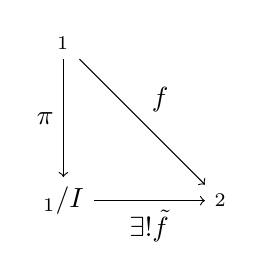
\begin{tikzpicture}[node distance = 2cm]
     \node (g1) {$\g_1$};
     \node (gI) [below of = g1] {$\g_1/I$};
     \node (g2) [right of = gI] {$\g_2$};
     \draw[->] (g1) to node[above right] {$f$} (g2);
     \draw[->] (g1) to node[left] {$\pi$} (gI);
     \draw[->] (gI) to node[below] {$\exists! \tilde{f}$} (g2);
    \end{tikzpicture}
   \end{center}
 \end{enumerate}
\end{prop}











































